%%%%%%%%%%%%%%%%%%%%%%%%%%%%%%%%%%%%%%%%%%%%%%%%%%%%%%%%%%%%%%%%%%%%%%%%%%%%%%%
% Three small transiting planet candidates from TESS around TOI-678, GJ 237
% (HIP 31126) and TOI-5997. Open Journal of Astrophysics research article.
% Derived numbers are macros from numbers.tex (and rows of tab_*.tex), written
% by scripts/s08_make_numbers.py from the analysis outputs.
% Build: pdflatex; bibtex; pdflatex; pdflatex  (openjournal.cls, aasjournal.bst).
%%%%%%%%%%%%%%%%%%%%%%%%%%%%%%%%%%%%%%%%%%%%%%%%%%%%%%%%%%%%%%%%%%%%%%%%%%%%%%%
\documentclass[twocolumn,numberedappendix,appendixfloats]{openjournal}

\usepackage{graphicx}
\graphicspath{{../figures/}{./}}
\usepackage{amsmath}
\usepackage{txfonts}
\usepackage[colorlinks,citecolor=blue,linkcolor=blue,urlcolor=blue,hypertexnames=false]{hyperref}
\usepackage{array}
\newcolumntype{L}[1]{>{\raggedright\arraybackslash}p{#1}}
\newcommand{\rearth}{R_{\oplus}}
\newcommand{\mearth}{M_{\oplus}}
\newcommand{\rsun}{R_{\odot}}
\newcommand{\msun}{M_{\odot}}
\newcommand{\lsun}{L_{\odot}}
\newcommand{\gcc}{\,\mathrm{g\,cm^{-3}}}
\newcommand{\tablefoot}[1]{\par\vspace{3pt}{\footnotesize\raggedright #1\par}}
\providecommand{\jatis}{J.~Astron. Telesc. Instrum. Syst.}
\providecommand{\rnaas}{Res. Notes AAS}
\providecommand{\psj}{PSJ}
\providecommand{\fass}{Front. Astron. Space Sci.}
\providecommand{\icarus}{Icarus}
% generated by scripts/s08_make_numbers.py -- do not edit
\newcommand{\FPPHp}{0.40 \pm 0.02}
\newcommand{\FPPTf}{(3.7 \pm 0.2)\times10^{-4}}
\newcommand{\FPPTfb}{5.1\times10^{-4}}
\newcommand{\FPPTs}{0.021 \pm 0.002}
\newcommand{\FPPTsb}{0.0039}
\newcommand{\FPPpixHp}{0.41}
\newcommand{\FPPpixTf}{\text{as adopted}}
\newcommand{\FPPpixTs}{\text{as adopted}}
\newcommand{\FPPtessHp}{0.63}
\newcommand{\FPPtessTf}{0.051}
\newcommand{\FPPtessTs}{0.025}
\newcommand{\GHp}{10.02}
\newcommand{\GHpB}{11.60}
\newcommand{\GTf}{9.90}
\newcommand{\GTs}{11.40}
\newcommand{\GaiaHp}{5568872394338114560}
\newcommand{\GaiaHpB}{5568872398635858816}
\newcommand{\GaiaTf}{4602034956332491264}
\newcommand{\GaiaTs}{5490097505810081024}
\newcommand{\JHp}{7.63}
\newcommand{\JTf}{8.32}
\newcommand{\JTs}{10.26}
\newcommand{\KHp}{1.3}
\newcommand{\KHpB}{2.4}
\newcommand{\KTf}{0.7}
\newcommand{\KTs}{1.6}
\newcommand{\KsHp}{6.79}
\newcommand{\KsTf}{7.68}
\newcommand{\KsTs}{9.85}
\newcommand{\LsHp}{0.069 \pm 0.009}
\newcommand{\LsHpB}{0.0219 \pm 0.0032}
\newcommand{\LsTf}{0.211 \pm 0.007}
\newcommand{\LsTs}{1.00 \pm 0.02}
\newcommand{\MKsoffHp}{0.22}
\newcommand{\MpHp}{4.2}
\newcommand{\MpHpB}{6.3}
\newcommand{\MpTf}{2.2}
\newcommand{\MpTs}{12.7}
\newcommand{\MsHp}{0.578 \pm 0.019}
\newcommand{\MsHpB}{0.404 \pm 0.018}
\newcommand{\MsTf}{0.686 \pm 0.053}
\newcommand{\MsTs}{1.036 \pm 0.086}
\newcommand{\NFPPHp}{0.40 \pm 0.02}
\newcommand{\NFPPTf}{(3.4 \pm 0.3)\times10^{-4}}
\newcommand{\NFPPTfb}{8.8\times10^{-5}}
\newcommand{\NFPPTs}{0.016 \pm 0.002}
\newcommand{\NFPPTsb}{0.0037}
\newcommand{\NFPPpixHp}{0.40}
\newcommand{\NFPPpixTf}{\text{as adopted}}
\newcommand{\NFPPpixTs}{\text{as adopted}}
\newcommand{\NFPPtessHp}{0.44}
\newcommand{\NFPPtessTf}{3.2\times10^{-4}}
\newcommand{\NFPPtessTs}{0.0089}
\newcommand{\PHp}{29.28559 \pm 0.00006}
\newcommand{\PHpB}{29.28558 \pm 0.00006}
\newcommand{\PHpfx}{14.810}
\newcommand{\PTf}{14.21604 \pm 0.00005}
\newcommand{\PTfb}{5.654997 \pm 0.000012}
\newcommand{\PTfbx}{5.655}
\newcommand{\PTs}{130.1455 \pm 0.0007}
\newcommand{\PTsb}{11.329893 \pm 0.000013}
\newcommand{\PTsbx}{11.330}
\newcommand{\PTstx}{6.562}
\newcommand{\PshortHp}{29.286}
\newcommand{\PshortHpB}{29.286}
\newcommand{\PshortTf}{14.216}
\newcommand{\PshortTs}{130.145}
\newcommand{\RpHp}{1.88 \pm 0.11}
\newcommand{\RpHpB}{2.39 \pm 0.14}
\newcommand{\RpTf}{1.27 \pm 0.09}
\newcommand{\RpTfb}{1.44 \pm 0.11}
\newcommand{\RpTs}{3.60 \pm 0.28}
\newcommand{\RpTsb}{3.33 \pm 0.21}
\newcommand{\RprHp}{1.9}
\newcommand{\RprHpB}{2.4}
\newcommand{\RprTf}{1.3}
\newcommand{\RprTs}{3.6}
\newcommand{\RsHp}{0.588 \pm 0.025}
\newcommand{\RsHpB}{0.411 \pm 0.018}
\newcommand{\RsTf}{0.687 \pm 0.042}
\newcommand{\RsTs}{1.088 \pm 0.066}
\newcommand{\RxcheckpctHp}{7}
\newcommand{\SHp}{2.9 \pm 0.4}
\newcommand{\SHpB}{1.16 \pm 0.17}
\newcommand{\STf}{21 \pm 1}
\newcommand{\STs}{3.9 \pm 0.2}
\newcommand{\SrHp}{2.9}
\newcommand{\SrHpB}{1.2}
\newcommand{\SrTf}{20.5}
\newcommand{\SrTs}{3.9}
\newcommand{\TTsm}{17.8}
\newcommand{\TTsn}{16.5}
\newcommand{\TTso}{17.9}
\newcommand{\TTsp}{15.7}
\newcommand{\TTsq}{12.8}
\newcommand{\TdurHp}{2.14 \pm 0.07}
\newcommand{\TdurHpB}{2.17 \pm 0.07}
\newcommand{\TdurTf}{3.16 \pm 0.12}
\newcommand{\TdurTfb}{1.68 \pm 0.05}
\newcommand{\TdurTs}{6.05 \pm 0.21}
\newcommand{\TdurTsb}{4.23 \pm 0.05}
\newcommand{\TdurboxHp}{2.0}
\newcommand{\TdurboxTf}{3.1}
\newcommand{\TdurboxTs}{6.4}
\newcommand{\TdurrHp}{2.1}
\newcommand{\TdurrHpB}{2.2}
\newcommand{\TdurrTf}{3.2}
\newcommand{\TdurrTs}{6.1}
\newcommand{\TeffHp}{3864 \pm 99}
\newcommand{\TeffHpB}{3465 \pm 99}
\newcommand{\TeffTf}{4717 \pm 106}
\newcommand{\TeffTs}{5536 \pm 148}
\newcommand{\TeqHp}{363 \pm 12}
\newcommand{\TeqHpB}{289 \pm 11}
\newcommand{\TeqTf}{593 \pm 9}
\newcommand{\TeqTs}{391 \pm 6}
\newcommand{\TeqrHp}{363}
\newcommand{\TeqrHpB}{289}
\newcommand{\TeqrTf}{593}
\newcommand{\TeqrTs}{391}
\newcommand{\TmagHpA}{9.13}
\newcommand{\TmagHpB}{10.55}
\newcommand{\TzHp}{3334.9927 \pm 0.0018}
\newcommand{\TzHpB}{3334.9926 \pm 0.0016}
\newcommand{\TzTf}{2758.2834^{+0.0022}_{-0.0032}}
\newcommand{\TzTs}{2972.2556 \pm 0.0048}
\newcommand{\aHp}{0.155 \pm 0.002}
\newcommand{\aHpB}{0.137 \pm 0.002}
\newcommand{\aTf}{0.101 \pm 0.003}
\newcommand{\aTs}{0.509 \pm 0.014}
\newcommand{\aliasminHp}{8}
\newcommand{\aliasminTf}{5}
\newcommand{\aliasminTs}{8}
\newcommand{\aliasworstHp}{0.6}
\newcommand{\aliasworstTf}{0.8}
\newcommand{\aliasworstTs}{0.7}
\newcommand{\aprojAB}{79}
\newcommand{\arsHp}{56.6 \pm 2.1}
\newcommand{\arsHpB}{72.3 \pm 2.5}
\newcommand{\arsTf}{32.9 \pm 1.9}
\newcommand{\arsTs}{104.7^{+2.4}_{-4.3}}
\newcommand{\bHp}{0.88 \pm 0.02}
\newcommand{\bHpB}{0.79 \pm 0.03}
\newcommand{\bTf}{0.33 \pm 0.20}
\newcommand{\bTfb}{0.75 \pm 0.04}
\newcommand{\bTs}{0.81 \pm 0.02}
\newcommand{\bTsb}{0.21 \pm 0.15}
\newcommand{\betaHp}{1.63}
\newcommand{\betaTf}{1.42}
\newcommand{\betaTs}{1.15}
\newcommand{\betacHp}{1.45}
\newcommand{\betacTf}{1.10}
\newcommand{\betacTs}{1.00}
\newcommand{\blindhiHp}{59}
\newcommand{\blindhiTf}{40}
\newcommand{\blindhiTs}{138}
\newcommand{\blindloHp}{19}
\newcommand{\blindloTf}{7}
\newcommand{\blindloTs}{69}
\newcommand{\blindnextHp}{14.1}
\newcommand{\blindnextTf}{10.5}
\newcommand{\blindnextTs}{9.0}
\newcommand{\blindpmaxHp}{60}
\newcommand{\blindpmaxTf}{40}
\newcommand{\blindpmaxTs}{150}
\newcommand{\blindsdeHp}{17.5}
\newcommand{\blindsdeTf}{11.8}
\newcommand{\blindsdeTs}{9.1}
\newcommand{\boxdepHp}{967 \pm 99}
\newcommand{\boxdepHpf}{1413 \pm 70}
\newcommand{\boxdepTf}{330 \pm 39}
\newcommand{\boxdepTfb}{337 \pm 29}
\newcommand{\boxdepTs}{869 \pm 90}
\newcommand{\boxdepTsb}{852 \pm 37}
\newcommand{\boxdepTst}{248 \pm 35}
\newcommand{\bprpHp}{1.91}
\newcommand{\bprpHpB}{2.42}
\newcommand{\bprpTf}{1.26}
\newcommand{\bprpTs}{0.92}
\newcommand{\chiscaleHp}{4.1}
\newcommand{\chiscaleHpf}{2.4}
\newcommand{\chiscaleTf}{4.4}
\newcommand{\chiscaleTfb}{2.7}
\newcommand{\chiscaleTs}{3.7}
\newcommand{\chiscaleTsb}{4.6}
\newcommand{\crowdHp}{0.592}
\newcommand{\crowdTf}{0.990}
\newcommand{\crowdTs}{0.892}
\newcommand{\crowdagree}{2}
\newcommand{\dchiHpA}{9.9}
\newcommand{\dchiHpB}{2.9}
\newcommand{\depAtrue}{0.75}
\newcommand{\depBtrue}{2.8}
\newcommand{\depHp}{856 \pm 75}
\newcommand{\depHpB}{2841 \pm 222}
\newcommand{\depTf}{289 \pm 24}
\newcommand{\depTs}{927 \pm 95}
\newcommand{\depfiveTf}{246 \pm 81}
\newcommand{\depfiveTfb}{233 \pm 52}
\newcommand{\depfivepctTfb}{31}
\newcommand{\deplateTsb}{671 \pm 73}
\newcommand{\deplatepctTsb}{21}
\newcommand{\distHp}{23.81 \pm 0.01}
\newcommand{\distHpB}{23.77 \pm 0.01}
\newcommand{\distTf}{46.62 \pm 0.03}
\newcommand{\distTs}{206.98 \pm 0.55}
\newcommand{\distrHp}{23.8}
\newcommand{\distrTf}{46.6}
\newcommand{\distrTs}{207.0}
\newcommand{\dplxAB}{0.072 \pm 0.019}
\newcommand{\dplxsigAB}{3.9}
\newcommand{\dpmAB}{21.7}
\newcommand{\dvtAB}{2.5}
\newcommand{\ebvTs}{0.045}
\newcommand{\evenHp}{1004 \pm 136}
\newcommand{\evenTf}{365 \pm 51}
\newcommand{\evenTs}{800 \pm 108}
\newcommand{\fABsig}{40}
\newcommand{\fAap}{0.76}
\newcommand{\fBap}{0.21}
\newcommand{\fehHp}{--}
\newcommand{\fehTf}{-0.34 \pm 0.08}
\newcommand{\fehTs}{0.10 \pm 0.08}
\newcommand{\ffiQ}{0.45^{+0.25}_{-0.25}}
\newcommand{\ffiQone}{2.0}
\newcommand{\ffiQsap}{1.48^{+0.38}_{-0.38}}
\newcommand{\ffiQsapone}{1.2}
\newcommand{\ffiQsapz}{3.8}
\newcommand{\ffiQz}{1.7}
\newcommand{\ffiS}{1.10^{+0.35}_{-0.35}}
\newcommand{\ffiSone}{0.3}
\newcommand{\ffiSsap}{0.98^{+0.27}_{-0.27}}
\newcommand{\ffiSsapone}{0.1}
\newcommand{\ffiSsapz}{3.3}
\newcommand{\ffiSz}{3.0}
\newcommand{\ffisix}{-0.15^{+0.15}_{-0.18}}
\newcommand{\ffisixQ}{-0.05^{+0.20}_{-0.22}}
\newcommand{\ffisixQone}{4.9}
\newcommand{\ffisixQz}{0.3}
\newcommand{\ffisixone}{6.8}
\newcommand{\ffisixz}{0.9}
\newcommand{\fmaxdurA}{3.3}
\newcommand{\fmaxdurB}{2.6}
\newcommand{\fsrcT}{13.4}
\newcommand{\fsrcTIC}{293689273}
\newcommand{\fsrcneed}{5.8}
\newcommand{\fsrcsep}{33}
\newcommand{\fsrcsig}{1.5}
\newcommand{\gA}{1.287}
\newcommand{\gB}{0.350}
\newcommand{\incHp}{89.11 \pm 0.05}
\newcommand{\incHpB}{89.38 \pm 0.04}
\newcommand{\incTf}{89.43 \pm 0.38}
\newcommand{\incTs}{89.56^{+0.02}_{-0.03}}
\newcommand{\insratio}{2.5}
\newcommand{\loggHp}{4.66 \pm 0.03}
\newcommand{\loggHpB}{4.82 \pm 0.03}
\newcommand{\loggTf}{4.60 \pm 0.08}
\newcommand{\loggTs}{4.38 \pm 0.08}
\newcommand{\loggspecTf}{4.62}
\newcommand{\loggspecTs}{4.34}
\newcommand{\nbTICTf}{1508332922}
\newcommand{\nbTTf}{17.1}
\newcommand{\nbootpix}{500}
\newcommand{\nbsepTf}{28}
\newcommand{\nbsigTf}{4.1}
\newcommand{\nbsigcTf}{2.5}
\newcommand{\nbxTHp}{15.5}
\newcommand{\nbxTHpf}{10.5}
\newcommand{\nbxTICHp}{293689268}
\newcommand{\nbxTICHpf}{293689267}
\newcommand{\nbxTICTfb}{1508332922}
\newcommand{\nbxTICTsb}{766625695}
\newcommand{\nbxTTfb}{17.1}
\newcommand{\nbxTTsb}{17.8}
\newcommand{\nbxneedHp}{27}
\newcommand{\nbxneedHpf}{0}
\newcommand{\nbxneedTfb}{50}
\newcommand{\nbxneedTsb}{58}
\newcommand{\nbxsepHp}{19}
\newcommand{\nbxsepHpf}{3}
\newcommand{\nbxsepTfb}{28}
\newcommand{\nbxsepTsb}{27}
\newcommand{\nbxsigHp}{5.7}
\newcommand{\nbxsigHpf}{40.0}
\newcommand{\nbxsigTfb}{8.0}
\newcommand{\nbxsigTsb}{5.7}
\newcommand{\nbxsigcHp}{3.6}
\newcommand{\nbxsigcHpf}{40.0}
\newcommand{\nbxsigcTfb}{3.9}
\newcommand{\nbxsigcTsb}{3.3}
\newcommand{\ncompTs}{5}
\newcommand{\needTsm}{59}
\newcommand{\needTsn}{18}
\newcommand{\needTso}{80}
\newcommand{\needTsp}{9}
\newcommand{\needTsq}{1.2}
\newcommand{\needmaxTs}{90}
\newcommand{\needminTs}{1}
\newcommand{\neffTs}{1105}
\newcommand{\nextTsa}{2026 December 29}
\newcommand{\nextTsb}{2027 May 8}
\newcommand{\nindepHp}{343}
\newcommand{\nindepTf}{111}
\newcommand{\nindepTs}{488}
\newcommand{\nnbHp}{5}
\newcommand{\nnbHpf}{5}
\newcommand{\nnbTf}{4}
\newcommand{\nnbTfb}{4}
\newcommand{\nnbTs}{9}
\newcommand{\nnbTsb}{9}
\newcommand{\nnbxHp}{4}
\newcommand{\nnbxHpf}{4}
\newcommand{\nnbxTf}{0}
\newcommand{\nnbxTfb}{4}
\newcommand{\nnbxTs}{0}
\newcommand{\nnbxTsb}{7}
\newcommand{\nnotxTs}{9}
\newcommand{\notxlistTs}{TIC~766625715, TIC~294395924, TIC~766625695, TIC~294395934, TIC~766625709, TIC~294395921, TIC~294395941, TIC~294395913, TIC~287276201}
\newcommand{\nrunHp}{5}
\newcommand{\nrunTf}{4}
\newcommand{\nrunTfb}{1}
\newcommand{\nrunTs}{5}
\newcommand{\nrunTsb}{1}
\newcommand{\nrunpixHp}{1}
\newcommand{\nrunpixTf}{0}
\newcommand{\nrunpixTs}{0}
\newcommand{\nruntessHp}{1}
\newcommand{\nruntessTf}{1}
\newcommand{\nruntessTs}{1}
\newcommand{\nseasHp}{4}
\newcommand{\nseasTf}{3}
\newcommand{\nseasTs}{3}
\newcommand{\nsecHp}{8}
\newcommand{\nsecTf}{6}
\newcommand{\nsecTs}{18}
\newcommand{\nshiftcolHp}{0.2}
\newcommand{\nshiftcolTf}{0.6}
\newcommand{\nshiftcolTs}{-0.1}
\newcommand{\nshiftrowHp}{0.3}
\newcommand{\nshiftrowTf}{-0.9}
\newcommand{\nshiftrowTs}{0.1}
\newcommand{\ntauHp}{56}
\newcommand{\ntauHpB}{63}
\newcommand{\ntauTf}{38}
\newcommand{\ntauTs}{23}
\newcommand{\ntaufreeHp}{13}
\newcommand{\ntaufreeTf}{15}
\newcommand{\ntaufreeTs}{16}
\newcommand{\ntaumax}{63}
\newcommand{\ntaumin}{23}
\newcommand{\ntrHp}{7}
\newcommand{\ntrHpf}{11}
\newcommand{\ntrTf}{9}
\newcommand{\ntrTfb}{20}
\newcommand{\ntrTs}{3}
\newcommand{\ntrTsb}{32}
\newcommand{\ntrTst}{50}
\newcommand{\ntransarchive}{4\,740}
\newcommand{\nullnHp}{3\,000}
\newcommand{\nullnTf}{3\,000}
\newcommand{\nullnTs}{3\,000}
\newcommand{\nullzHp}{9.7}
\newcommand{\nullzHpf}{18.1}
\newcommand{\nullzTf}{7.5}
\newcommand{\nullzTfb}{11.3}
\newcommand{\nullzTs}{8.5}
\newcommand{\nullzTsb}{19.0}
\newcommand{\nullzTst}{7.5}
\newcommand{\oddHp}{914 \pm 145}
\newcommand{\oddTf}{292 \pm 60}
\newcommand{\oddTs}{982 \pm 161}
\newcommand{\oeHp}{0.5}
\newcommand{\oeHpf}{2.4}
\newcommand{\oeTf}{0.9}
\newcommand{\oeTfb}{0.7}
\newcommand{\oeTs}{0.9}
\newcommand{\oeTsb}{2.0}
\newcommand{\oeTst}{1.2}
\newcommand{\offHp}{-1.4, -4.5}
\newcommand{\offHpf}{+3.2, -33.6}
\newcommand{\offTf}{+0.0, -5.4}
\newcommand{\offTfb}{-1.0, +3.8}
\newcommand{\offTs}{-0.8, +2.9}
\newcommand{\offTsb}{-8.8, -4.9}
\newcommand{\offsdHp}{3.3, 3.5}
\newcommand{\offsdHpf}{0.3, 0.4}
\newcommand{\offsdTf}{6.0, 5.5}
\newcommand{\offsdTfb}{3.8, 3.8}
\newcommand{\offsdTs}{6.9, 4.6}
\newcommand{\offsdTsb}{6.5, 3.5}
\newcommand{\pBTPHp}{(0.0 \pm 0.0)\times10^{-12}}
\newcommand{\pBTPTf}{(0.0 \pm 0.0)\times10^{-12}}
\newcommand{\pBTPTs}{(0.0 \pm 0.0)\times10^{-12}}
\newcommand{\pEBHp}{0.0174 \pm 0.0018}
\newcommand{\pEBTf}{(3.3 \pm 0.3)\times10^{-4}}
\newcommand{\pEBTs}{0.012 \pm 0.002}
\newcommand{\pEBmaxHp}{0.02}
\newcommand{\pEBmaxTf}{4\times10^{-4}}
\newcommand{\pEBmaxTs}{0.02}
\newcommand{\pEBpixHp}{4.8\times10^{-4}}
\newcommand{\pEBpixmaxHp}{5\times10^{-4}}
\newcommand{\pNTPBHp}{0.38 \pm 0.02}
\newcommand{\pNTPHp}{0.38 \pm 0.02}
\newcommand{\pNTPTf}{(5.5 \pm 1.2)\times10^{-6}}
\newcommand{\pNTPTs}{0.0050 \pm 0.0008}
\newcommand{\pSTPHp}{0.0031 \pm 0.0003}
\newcommand{\pSTPTf}{(2.8 \pm 3.0)\times10^{-5}}
\newcommand{\pSTPTs}{0.0033 \pm 0.0013}
\newcommand{\perratioTf}{2.514}
\newcommand{\perresoffTf}{0.6}
\newcommand{\pixdetHp}{11}
\newcommand{\pixdetHpf}{104}
\newcommand{\pixdetTf}{7}
\newcommand{\pixdetTfb}{7}
\newcommand{\pixdetTs}{6}
\newcommand{\pixdetTsb}{8}
\newcommand{\pixdetcHp}{5.1}
\newcommand{\pixdetcHpf}{inf}
\newcommand{\pixdetcTf}{2.7}
\newcommand{\pixdetcTfb}{4.2}
\newcommand{\pixdetcTs}{2.7}
\newcommand{\pixdetcTsb}{3.5}
\newcommand{\pixsigHp}{0.8}
\newcommand{\pixsigHpBstar}{0.2}
\newcommand{\pixsigHpf}{40.0}
\newcommand{\pixsigTf}{0.5}
\newcommand{\pixsigTfb}{0.6}
\newcommand{\pixsigTs}{0.3}
\newcommand{\pixsigTsb}{1.1}
\newcommand{\pixsigcHp}{1.0}
\newcommand{\pixsigcHpBstar}{0.4}
\newcommand{\pixsigcHpf}{40.0}
\newcommand{\pixsigcTf}{0.7}
\newcommand{\pixsigcTfb}{0.7}
\newcommand{\pixsigcTs}{0.2}
\newcommand{\pixsigcTsb}{1.6}
\newcommand{\plxHp}{41.991 \pm 0.012}
\newcommand{\plxHpB}{42.063 \pm 0.015}
\newcommand{\plxTf}{21.450 \pm 0.012}
\newcommand{\plxTs}{4.831 \pm 0.013}
\newcommand{\pmHp}{-277.53, -29.76}
\newcommand{\pmHpB}{-263.67, -13.04}
\newcommand{\pmTf}{-223.52, +177.32}
\newcommand{\pmTs}{-31.33, +71.64}
\newcommand{\pnbqTs}{0.013 \pm 0.002}
\newcommand{\pplanetHp}{0.60 \pm 0.02}
\newcommand{\pplanetTf}{0.99963 \pm 0.00002}
\newcommand{\pplanetTs}{0.979 \pm 0.002}
\newcommand{\psysHp}{0.9826 \pm 0.0018}
\newcommand{\psysTf}{0.99966 \pm 0.00003}
\newcommand{\psysTs}{0.983 \pm 0.002}
\newcommand{\ptchiHp}{2.3}
\newcommand{\ptchiTf}{9.1}
\newcommand{\ptchiTs}{2.8}
\newcommand{\ptchicHp}{2.9}
\newcommand{\ptchicTf}{15.0}
\newcommand{\ptchicTs}{3.7}
\newcommand{\ptdepaTs}{982 \pm 161}
\newcommand{\ptdepbTs}{942 \pm 149}
\newcommand{\ptdepcTs}{640 \pm 158}
\newcommand{\ptdofHp}{6}
\newcommand{\ptdofTf}{8}
\newcommand{\ptdofTs}{2}
\newcommand{\ptpHp}{0.89}
\newcommand{\ptpHpf}{0.86}
\newcommand{\ptpTf}{0.34}
\newcommand{\ptpTfb}{0.51}
\newcommand{\ptpTs}{0.25}
\newcommand{\ptpTsb}{0.014}
\newcommand{\ptpTst}{0.87}
\newcommand{\ptpcHp}{0.82}
\newcommand{\ptpcTf}{0.06}
\newcommand{\ptpcTs}{0.16}
\newcommand{\qoneHp}{0.41 \pm 0.15}
\newcommand{\qoneTf}{0.41 \pm 0.13}
\newcommand{\qoneTs}{0.26 \pm 0.13}
\newcommand{\qtwoHp}{0.26 \pm 0.13}
\newcommand{\qtwoTf}{0.33 \pm 0.15}
\newcommand{\qtwoTs}{0.23 \pm 0.14}
\newcommand{\radratio}{1.27}
\newcommand{\rhofitHp}{4.00 \pm 0.45}
\newcommand{\rhofitHpB}{8.33 \pm 0.86}
\newcommand{\rhofitTf}{3.35 \pm 0.57}
\newcommand{\rhofitTs}{1.28^{+0.09}_{-0.15}}
\newcommand{\rhofreeHp}{17.8^{+14.0}_{-13.2}}
\newcommand{\rhofreeTf}{2.7^{+1.3}_{-1.9}}
\newcommand{\rhofreeTs}{3.8^{+2.1}_{-2.6}}
\newcommand{\rhofreesigHpA}{1.0}
\newcommand{\rhofreesigHpB}{0.7}
\newcommand{\rhofreesigTf}{0.2}
\newcommand{\rhofreesigTs}{1.0}
\newcommand{\rhopriorHp}{4.00 \pm 0.44}
\newcommand{\rhopriorTf}{2.98 \pm 0.69}
\newcommand{\rhopriorTs}{1.13 \pm 0.27}
\newcommand{\rhosHp}{4.00 \pm 0.44}
\newcommand{\rhosHpB}{8.19 \pm 0.90}
\newcommand{\rhosTf}{2.98 \pm 0.69}
\newcommand{\rhosTs}{1.13 \pm 0.27}
\newcommand{\rmsHp}{1066}
\newcommand{\rmsTf}{713}
\newcommand{\rmsTs}{1662}
\newcommand{\rprsHp}{0.0293 \pm 0.0013}
\newcommand{\rprsHpB}{0.0533 \pm 0.0021}
\newcommand{\rprsTf}{0.0170 \pm 0.0007}
\newcommand{\rprsTs}{0.0304 \pm 0.0016}
\newcommand{\ruweHp}{1.01}
\newcommand{\ruweHpB}{0.98}
\newcommand{\ruweTf}{1.03}
\newcommand{\ruweTs}{0.90}
\newcommand{\rvHp}{--}
\newcommand{\rvHpB}{+11.0 \pm 0.3}
\newcommand{\rvTf}{-27.2 \pm 0.2}
\newcommand{\rvTs}{+40.1 \pm 0.4}
\newcommand{\rvampHp}{--}
\newcommand{\rvampTf}{1.7}
\newcommand{\rvampTs}{5.3}
\newcommand{\rvpHp}{--}
\newcommand{\rvpHpB}{0.92}
\newcommand{\rvpTf}{0.10}
\newcommand{\rvpTs}{0.28}
\newcommand{\sapHp}{527 \pm 59}
\newcommand{\sapTf}{349 \pm 43}
\newcommand{\sapTs}{719 \pm 84}
\newcommand{\sapcHp}{889 \pm 99}
\newcommand{\sapcTf}{353 \pm 43}
\newcommand{\sapcTs}{806 \pm 94}
\newcommand{\seachiHp}{1.0}
\newcommand{\seachiTf}{1.4}
\newcommand{\seachiTs}{2.8}
\newcommand{\seachicHp}{1.3}
\newcommand{\seachicTf}{2.4}
\newcommand{\seachicTs}{3.7}
\newcommand{\seadofHp}{3}
\newcommand{\seadofTf}{2}
\newcommand{\seadofTs}{2}
\newcommand{\seapHp}{0.79}
\newcommand{\seapHpf}{0.68}
\newcommand{\seapTf}{0.49}
\newcommand{\seapTfb}{0.049}
\newcommand{\seapTs}{0.25}
\newcommand{\seapTsb}{0.015}
\newcommand{\seapTst}{0.69}
\newcommand{\seapcHp}{0.73}
\newcommand{\seapcTf}{0.30}
\newcommand{\seapcTs}{0.16}
\newcommand{\secHp}{-216 \pm 90}
\newcommand{\secTf}{41 \pm 50}
\newcommand{\secTs}{-209 \pm 96}
\newcommand{\secmaxHp}{2.6}
\newcommand{\secmaxTf}{2.9}
\newcommand{\secmaxTs}{3.2}
\newcommand{\secmaxphHp}{0.32}
\newcommand{\secmaxphTf}{0.42}
\newcommand{\secmaxphTs}{0.42}
\newcommand{\sepAB}{3.33}
\newcommand{\sepTsm}{27}
\newcommand{\sepTsn}{19}
\newcommand{\sepTso}{34}
\newcommand{\sepTsp}{20}
\newcommand{\sepTsq}{33}
\newcommand{\sigTsm}{3.2}
\newcommand{\sigTsn}{3.7}
\newcommand{\sigTso}{4.6}
\newcommand{\sigTsp}{3.9}
\newcommand{\sigTsq}{8.9}
\newcommand{\sigcTsm}{2.4}
\newcommand{\sigcTsn}{1.8}
\newcommand{\sigcTso}{2.7}
\newcommand{\sigcTsp}{1.9}
\newcommand{\sigcTsq}{2.7}
\newcommand{\sigtcHp}{8}
\newcommand{\sigtcTf}{10}
\newcommand{\sigtcTs}{16}
\newcommand{\snrHp}{11.0}
\newcommand{\snrHpf}{27.3}
\newcommand{\snrTf}{10.8}
\newcommand{\snrTfb}{12.0}
\newcommand{\snrTs}{11.1}
\newcommand{\snrTsb}{31.7}
\newcommand{\snrTst}{8.7}
\newcommand{\snrfullHp}{9.8}
\newcommand{\snrfullHpf}{20.2}
\newcommand{\snrfullTf}{8.4}
\newcommand{\snrfullTfb}{11.6}
\newcommand{\snrfullTs}{9.7}
\newcommand{\snrfullTsb}{23.2}
\newcommand{\snrfullTst}{7.2}
\newcommand{\tenthTf}{2019.05}
\newcommand{\tenthdtTf}{1.0}
\newcommand{\twomassHp}{06315111-4332026}
\newcommand{\twomassTf}{17323692+3334108}
\newcommand{\twomassTs}{07171942-5535536}
\newcommand{\vorbAB}{3.3}
\newcommand{\xTsm}{no}
\newcommand{\xTsn}{no}
\newcommand{\xTso}{no}

\hyphenation{TRICERATOPS}
\hypersetup{pdftitle={Three small transiting planet candidates from TESS around TOI-678, GJ 237 and TOI-5997},
  pdfauthor={Samson Fraser}}
\renewcommand{\dbltopfraction}{0.9}
\renewcommand{\dblfloatpagefraction}{0.75}
\renewcommand{\topfraction}{0.9}
\renewcommand{\floatpagefraction}{0.75}
% openjournal.cls sets the float-to-text separations to -\baselineskip + 7mm with 10mm of
% shrink, which lets text run into the notes under wide tables on tight pages; use fixed gaps.
\setlength{\textfloatsep}{14pt plus 4pt minus 2pt}
\setlength{\dbltextfloatsep}{14pt plus 4pt minus 2pt}

\interfootnotelinepenalty=10000
\begin{document}

\title{Three small transiting planet candidates from TESS around TOI-678,
GJ\,237 and TOI-5997}

\author{Samson Fraser}
\email{samsonmfraser@gmail.com}
\affiliation{Independent researcher, Sicamous, British Columbia, Canada}
\submitted{Draft version \today}
\journalinfo{Prepared for The Open Journal of Astrophysics}

\begin{abstract}
We present three transiting planet candidates from TESS. Each was detected as a
threshold-crossing event (TCE) in the multi-sector searches of the TESS pipeline
but has not become a TESS Object of Interest (TOI). Around the G dwarf TOI-678, host of the candidate
TOI-678.01 (11.3\,d), three transits observed in 2019, 2023 and 2025 fix a
period of $\PshortTs$\,d and give a candidate of $\RpTs\,\rearth$ that receives
$\SrTs$ times the Earth's insolation. Around HIP~31126 (GJ\,237), a pair of early
M dwarfs $3.3''$ apart at 23.8\,pc, seven transits give a $\PshortHp$-d
candidate of $\RpHp\,\rearth$ if it orbits the primary or $\RpHpB\,\rearth$ if
it orbits the secondary. Around the K dwarf TOI-5997, host of the validated
planet TOI-5997\,b (5.65\,d), nine transits give a $\PshortTf$-d candidate of
$\RpTf\,\rearth$. With a conservative allowance for correlated noise the
signals have S/N of $\snrfullTf$--$\snrfullHp$. Their depths agree from transit
to transit and season to season, in simple-aperture as well as corrected
photometry, and none shows an odd--even difference, a secondary eclipse or a
period alias. A fit of the TESS pixel response function to difference images
places each source within about $1\sigma$ of its target. The same method places
a 14.8-d community TOI in the HIP~31126 field on a neighbour $33''$ away, which
is most likely an eclipsing binary. With archival speckle and adaptive-optics imaging, TRICERATOPS gives
false-positive probabilities of $\FPPTs$ for TOI-678 and $\FPPTf$ for
TOI-5997, the latter below the usual threshold for statistical validation. For HIP~31126 the value is $\FPPHp$, almost entirely because the
host star is unknown: eclipsing-binary scenarios carry $\pEBHp$ of the
probability. We present the three as planet candidates and give the transit
times and observations that would validate them.
\end{abstract}

\begin{keywords}
{planets and satellites: detection -- techniques: photometric -- binaries:
visual -- stars: individual: TOI-678, HIP 31126, TOI-5997 -- methods:
statistical}
\end{keywords}

\maketitle

%%%%%%%%%%%%%%%%%%%%%%%%%%%%%%%%%%%%%%%%%%%%%%%%%%%%%%%%%%%%%%%%%%%%%%%%%%%%%%%
\section{Introduction}
\label{sec:intro}

The Transiting Exoplanet Survey Satellite \citep[TESS;][]{ricker2015} has
observed most of the sky for more than eight years. The Science Processing
Operations Center (SPOC) pipeline \citep{jenkins2016} searches the 2-min light
curves of pre-selected stars sector by sector and, every few months, in
multi-sector runs that combine all sectors observed so far. A periodic signal
above the detection threshold becomes a threshold-crossing event (TCE), which
the Data Validation module \citep{twicken2018,li2019} fits and tests. TCEs that
the TESS team judges planetary become TESS Objects of Interest
\citep[TOIs;][]{guerrero2021}.

Long-period and shallow signals reach the threshold only after many sectors,
so they often first appear in the latest multi-sector run, whose TCE tables are
public before TOI vetting. Machine-learning classification of TCEs
\citep{valizadegan2025}, independent searches of the light curves
\citep{lafarga2026} and uniform statistical validation of TOIs
\citep{collier2026} show how much remains to be done with these data. Systems
that already host a candidate deserve particular attention: a second
transiting candidate on the same star is much less likely to be a false
positive than an isolated one \citep{lissauer2012}, and its host often already
has the high-resolution imaging and spectroscopy that a validation needs.

Here we present three TCEs from these multi-sector runs. Two lie on stars that already
host a planet or candidate: a 130-d signal on TOI-678 and a 14.2-d signal on
TOI-5997. The third, a 29.3-d signal, lies on HIP~31126 (GJ\,237), a nearby
pair of M dwarfs. None is a TOI or a community TOI (CTOI). The 14.2-d signal of
TOI-5997 was listed independently as a candidate in a public GitHub repository
on 2026 October 8 \citep{eumemic2026}. The HIP~31126 signal appears in the same
repository's table of vetted signals, flagged because of a close neighbour, but
is not listed as a candidate. We have not found any of the three signals in the literature.

Sections~\ref{sec:data} and \ref{sec:stars} describe the data and the stars,
Sect.~\ref{sec:methods} the analysis, Sect.~\ref{sec:results} the results for
each system and Sect.~\ref{sec:disc} what would validate the candidates. We
refer to the signals by host and period. If validated they would become
TOI-678\,c (or b), HIP~31126\,(A or B)\,b and TOI-5997\,c; we do not use these
letters, which are reserved for validated planets.

%%%%%%%%%%%%%%%%%%%%%%%%%%%%%%%%%%%%%%%%%%%%%%%%%%%%%%%%%%%%%%%%%%%%%%%%%%%%%%%
\section{Data}
\label{sec:data}

\subsection{TESS photometry and pipeline detections}
\label{sec:tess}

We used the SPOC 2-min Presearch Data Conditioning simple-aperture photometry
\citep[PDCSAP;][]{smith2012,stumpe2012} of every sector in which each star was
observed at 2-min cadence (Table~\ref{tab:data}). From the same sectors we
also used the simple-aperture photometry (SAP), flux-weighted centroids,
quality flags and target pixel files (TPFs). All data come from the Mikulski
Archive for Space Telescopes (MAST).

All three signals are SPOC detections. The TOI-678 signal (SPOC period
130.146\,d) and the HIP~31126 signal (29.286\,d) are TCEs of the multi-sector search of Sectors
1--96, with pipeline signal-to-noise ratios (S/N) of 9.6 and 10.8 and
multiple-event statistics of 8.7 and 9.5. For TOI-678 that run contains all
three transits; the first two had already been detected in the runs of
Sectors 1--65 and 1--69 as a two-transit TCE, with a period equal to their
1431.6-d spacing. For HIP~31126 it contains five of the seven transits used here; the
other two are in Sector 98. The 14.216-d signal of TOI-5997 is a TCE of the
search of Sectors 14--86 (S/N 11.3, multiple-event statistic 8.9). None of the
three has become a TOI. For the HIP~31126 TCE, the Data Validation
difference-image centroid lies $5.2 \pm 4.3''$ from the catalogue position of
the brighter star, HIP~31126\,A; for the TOI-678 TCE, Data Validation gave no
centroid result.

\begin{table*}
\caption{TESS 2-min data used.}
\label{tab:data}
\centering
\footnotesize
\begin{tabular}{lL{7.4cm}ccc}
\hline\hline
Star & Sectors & Transits used & CROWDSAP & 2-min scatter (ppm) \\
\hline
TOI-678 & 7, 8, 9, 30, 33, 34, 35, 36, 61, 62, 67, 69, 87, 88, 89, 90, 94, 96 & \ntrTs\ (S8, S61, S90) & \crowdTs & \rmsTs \\
HIP 31126 & 6, 7, 33, 34, 61, 87, 88, 98 & \ntrHp & \crowdHp & \rmsHp \\
TOI-5997 & 25, 26, 52, 53, 79, 80 & \ntrTf\ (+1) & \crowdTf & \rmsTf \\
\hline
\end{tabular}
\tablefoot{CROWDSAP is the SPOC estimate of the fraction of the flux in the
aperture that comes from the target, averaged over sectors. The scatter is
1.4826 times the median absolute deviation of the detrended 2-min flux.
Transits used are those with at least 60\% of the in-transit and of the
surrounding out-of-transit cadences. HIP~31126 has an eighth, partial transit
at the end of Sector 6, and TOI-5997 a tenth that overlaps a transit of
TOI-5997\,b (Sect.~\ref{sec:toi5997}).}
\end{table*}

\subsection{High-resolution imaging}
\label{sec:imaging}

All three stars have archival high-resolution imaging on the Exoplanet
Follow-up Observing Program website (ExoFOP). HIP~31126 was observed with the
speckle camera HRCam on the 4.1-m SOAR telescope in the $I$ band on 2019 May 18
\citep{tokovinin2018,ziegler2020}. The image resolves the companion B at
$3.26''$ (position angle $219^\circ$, $\Delta I = 1.5$) and shows no other
source; the $5\sigma$ limits relative to A, which we digitised from the
sensitivity curve posted with the data, are $\Delta I = 2.5$ at $0.15''$ and
5.4 at $1''$. TOI-678 was observed with the Zorro speckle imager on
Gemini-South at 562 and 832\,nm on 2020 December 28 and 2023 March 4
\citep{howell2011,scott2021}; we use the 2020 curves, the only ones posted as tables,
which reach $\Delta m_{832} = 4.8$ at $0.1''$ and 6.6 at $1''$. TOI-5997 was
observed with {`}Alopeke on Gemini-North at 562 and 832\,nm on 2024 May 23
($\Delta m_{832} = 7.2$ at $0.5''$) and with PHARO \citep{hayward2001} on the
Palomar 5-m telescope in Br$\gamma$ on 2023 June 6. No source other than
HIP~31126\,B was reported near any of the targets. An observation of TOI-5997
with the SAI 2.5-m speckle polarimeter is also on ExoFOP, without a tabulated
contrast curve; we do not use it.

\subsection{Spectroscopy and astrometry}
\label{sec:spec}

ExoFOP lists stellar parameters from CHIRON \citep{tokovinin2013} spectra of
TOI-678 taken at two epochs in 2019 and from two TRES spectra of TOI-5997 taken
in 2023, analysed with the Stellar Parameter Classification code
\citep[SPC;][]{buchhave2012}; TOI-678 also has two CORALIE \citep{queloz2000}
spectra from 2019. No radial velocities from these spectra are public. Gaia DR3
\citep{gaia2016,gaia2023} measured the radial velocities of TOI-678, TOI-5997
and HIP~31126\,B over 12--20 epochs \citep{katz2023} and found no variability
(probabilities of constancy $p = \rvpTs$, $\rvpTf$ and $\rvpHpB$). All three
targets and HIP~31126\,B have renormalised unit weight errors
\citep[RUWE;][]{lindegren2021} between 0.90 and 1.03 and no non-single-star
solution. We also
use 2MASS photometry \citep{skrutskie2006}.

%%%%%%%%%%%%%%%%%%%%%%%%%%%%%%%%%%%%%%%%%%%%%%%%%%%%%%%%%%%%%%%%%%%%%%%%%%%%%%%
\section{The stars}
\label{sec:stars}

Table~\ref{tab:stars} lists the stellar parameters.

For TOI-678 and TOI-5997 we computed the luminosity from the Gaia $G$
magnitude, the parallax and the bolometric correction of \citet{andrae2018},
with $E(B-V) = \ebvTs$ for TOI-678 and none for TOI-5997. We took $T_{\rm
eff}$, $\log g$ and [M/H] from the spectra, with $T_{\rm eff}$ uncertainties
of at least 2\% \citep{tayar2022}. We derived the radius from the
Stefan--Boltzmann law and the mass from the relations of \citet{torres2010},
which take the spectroscopic $T_{\rm eff}$, $\log g$ and [M/H] as input. The
$\log g$ implied by mass and radius agrees with the spectroscopic values ($\loggspecTs$ and $\loggspecTf$).
TOI-678 is a slightly metal-rich G7--G8 dwarf at 207\,pc; TOI-5997 is a
metal-poor K3--K4 dwarf at 46.6\,pc.

The proper motions of HIP~31126 A and B differ by
$\dpmAB$\,mas\,yr$^{-1}$, or $\dvtAB$\,km\,s$^{-1}$ at their distance. This is
less than the orbital speed of $\vorbAB$\,km\,s$^{-1}$ for a circular orbit at
their projected separation of $\aprojAB$\,au ($\sepAB''$ at the Gaia epoch 2016.0). Their
parallaxes differ by $\dplxAB$\,mas, formally $\dplxsigAB\sigma$, but
Gaia parallax uncertainties are underestimated for pairs this close
\citep{elbadry2021}. The
pair is consistent with being bound, and we treat it so. Its 2MASS photometry
is partly blended: B has a poor-quality $K_s$ measurement, and A's catalogued
$K_s$ is $\MKsoffHp$\,mag brighter than its Gaia photometry predicts, as
expected if it includes some of B's light. We therefore derived both stars'
parameters from Gaia. We converted the absolute magnitude $M_G$ into $M_{K_s}$
and $T_{\rm eff}$ with the dwarf sequence of \citet{pecaut2013}, in its updated
online version\footnote{Version 2022.04.16 of
\url{https://www.pas.rochester.edu/~emamajek/EEM_dwarf_UBVIJHK_colors_Teff.txt}.}
(uncertainties 0.1\,mag and 100\,K), and then obtained the radius from the radius--$M_{K_s}$
relation of \citet{mann2015}, the mass from the mass--$M_{K_s}$ relation of
\citet{mann2019}, and the luminosity from radius and $T_{\rm eff}$. Using A's catalogued $K_s$ instead would give a radius
$\RxcheckpctHp$\% larger. A and B are early M dwarfs, about M0 and M2.5.

The TESS Input Catalog lists B with $T = 9.53$, a magnitude brighter than its
Gaia photometry implies \citep[$T = \TmagHpB$ from the relations
of][]{stassun2019}, probably because the catalogue value comes from the
blended 2MASS photometry. The SPOC crowding correction used the catalogue
value, so the PDCSAP light curve of A over-corrects for B's light. We computed
the fraction of the flux in the SPOC aperture that comes from each star with
the TESS pixel response function (PRF) and the registered positions of all
catalogued stars (Sect.~\ref{sec:pixel}): A contributes $\fAap$ and B $\fBap$,
against the SPOC estimate of $\crowdHp$ for A. A transit on A therefore appears
in PDCSAP with $g_A = \gA$ times its true depth in A's light, and a transit on
B with $g_B = \gB$ times its depth in B's light. For TOI-678 and TOI-5997 our
flux fractions agree with the SPOC values to within $\crowdagree$\%.

\begin{table*}
\caption{Stellar parameters.}
\label{tab:stars}
\centering
\footnotesize
\begin{tabular}{lcccc}
\hline\hline
 & TOI-678 & HIP 31126 A & HIP 31126 B & TOI-5997 \\
\hline
Other names & TIC 294395926 & GJ 237, TIC 293689266 & TIC 293689267 & HIP 85850, TIC 39516274 \\
Gaia DR3 & \GaiaTs & \GaiaHp & \GaiaHpB & \GaiaTf \\
Parallax (mas) & $\plxTs$ & $\plxHp$ & $\plxHpB$ & $\plxTf$ \\
Distance (pc) & $\distTs$ & $\distHp$ & $\distHpB$ & $\distTf$ \\
$\mu_{\alpha*}, \mu_\delta$ (mas\,yr$^{-1}$) & $\pmTs$ & $\pmHp$ & $\pmHpB$ & $\pmTf$ \\
RUWE & \ruweTs & \ruweHp & \ruweHpB & \ruweTf \\
Gaia RV (km\,s$^{-1}$) & $\rvTs$ & -- & $\rvHpB$ & $\rvTf$ \\
$G$; $G_{BP}-G_{RP}$ (mag) & \GTs; \bprpTs & \GHp; \bprpHp & \GHpB; \bprpHpB & \GTf; \bprpTf \\
$T$ (mag) & 10.92 & \TmagHpA$^{a}$ & \TmagHpB$^{a}$ & 9.26 \\
$J$; $K_s$ (mag) & \JTs; \KsTs & \JHp; \KsHp$^{b}$ & blended & \JTf; \KsTf \\
$T_{\rm eff}$ (K) & $\TeffTs$ & $\TeffHp$ & $\TeffHpB$ & $\TeffTf$ \\
$\log g$ (cgs) & $\loggTs$ & $\loggHp$ & $\loggHpB$ & $\loggTf$ \\
$[{\rm M/H}]$ & $\fehTs$ & -- & -- & $\fehTf$ \\
$R_\star$ ($\rsun$) & $\RsTs$ & $\RsHp$ & $\RsHpB$ & $\RsTf$ \\
$M_\star$ ($\msun$) & $\MsTs$ & $\MsHp$ & $\MsHpB$ & $\MsTf$ \\
$\rho_\star$ ($\mathrm{g\,cm^{-3}}$) & $\rhosTs$ & $\rhosHp$ & $\rhosHpB$ & $\rhosTf$ \\
$L_\star$ ($\lsun$) & $\LsTs$ & $\LsHp$ & $\LsHpB$ & $\LsTf$ \\
\hline
\end{tabular}
\tablefoot{Astrometry and $G$ photometry from Gaia DR3; $J$, $K_s$ from 2MASS;
$T_{\rm eff}$ and [M/H] of TOI-678 and TOI-5997 from the CHIRON and TRES spectra
on ExoFOP; other parameters derived as described in Sect.~\ref{sec:stars}
($\log g$ from $M_\star$ and $R_\star$). $^{a}$From the Gaia colours
\citep{stassun2019}; the TIC lists 9.06 and 9.53. $^{b}$Probably includes some
light from B.}
\end{table*}

%%%%%%%%%%%%%%%%%%%%%%%%%%%%%%%%%%%%%%%%%%%%%%%%%%%%%%%%%%%%%%%%%%%%%%%%%%%%%%%
\section{Analysis}
\label{sec:methods}

The same code analysed all three systems. Four other signals in the same light
curves serve as controls: TOI-5997\,b, validated by \citet{collier2026};
TOI-678.01; a 6.56-d TCE of TOI-678; and a 14.8-d signal in the HIP~31126 light
curve that is listed as the CTOI TIC~293689267.01 (Appendix~\ref{app:controls}).
Before looking at the light curves, we fixed the criteria that a signal had to
meet. The main one was $\mathrm{S/N} \ge 10$, with correlated noise estimated by
the time-averaging method of Sect.~\ref{sec:vet}.

\subsection{Light curves}
\label{sec:lc}

We removed cadences with non-zero quality flags and detrended each sector with
a time-windowed biweight filter \citep{hippke2019} of width
$\max(0.75\,\mathrm{d}, 3T_{14})$, where $T_{14}$ is the transit duration,
with the transits of all known signals masked. Upward outliers more than five
times the robust scatter above the trend were removed. A second detrending,
with the same window and no masks, was used for blind searches.

\subsection{Tests of each signal}
\label{sec:vet}

The tests use a box-shaped measurement of the depth: the mean flux in the
central 80\% of the transit compared with the flux 1--3 transit durations on
either side. They use the ephemerides and durations of preliminary fits, which
differ from the final values (Table~\ref{tab:fit}) by at most 20\,min in
mid-transit time (for the earliest TOI-678 transit) and 6\% in duration; this
changes the box depths by a few per cent at most. We measured this depth at the candidate's ephemeris for all transits
together, per transit, per observing season, for odd and even transits, and in
SAP flux. We also measured it at phase 0.5, at every other phase of the orbit,
and at the extra epochs that periods of $P/2$ to $P/10$ would imply. We also searched each light curve with a box least-squares (BLS) periodogram
\citep{kovacs2002} up to a maximum period set for each star (Table~\ref{tab:vet}),
with trial durations of 0.6--1.3 times the candidate's and with the other known
signals masked. Finally, we measured the shift of the flux-weighted centroid in
transit.

Correlated noise enters through a factor $\beta$ by which the white-noise
uncertainties are multiplied. We estimated it in two ways. The full-phase
$\beta$ is the scatter of the depth S/N measured at every phase of the orbit
away from the transit. The time-averaging $\beta$ compares the scatter of the
out-of-transit residuals binned to the transit duration with the white-noise
expectation \citep{pont2006,winn2008}; it is floored at 1. The full-phase
value is the larger, and Table~\ref{tab:vet} gives the S/N and the consistency
tests with both. As a check that does not depend on a noise model, we compared
the depth at the candidate's ephemeris with the depths at 3000 randomly chosen
phases of the same period; because the boxes overlap, these correspond to only
$P/T_{14}$ (110--490) independent trials.

\subsection{Pixel-level localisation}
\label{sec:pixel}

The flux-weighted centroid is a blunt tool in crowded TESS apertures. To find
where each signal comes from, we fitted the TESS PRF to difference images, as
\citet{bryson2013} did for Kepler; \citet{higgins2023} use a related PRF fit to
locate variable stars in TESS data. For
every transit with full coverage in a 2-min TPF we subtracted the mean image in
transit (within $0.4\,T_{14}$ of mid-transit) from the mean of the images
0.75--1.75\,$T_{14}$ before and after it, and averaged the transits of each
sector. The same was done at 60 random epochs that avoid all known signals,
giving null difference images from which we estimated the per-pixel noise.

The PRF of each sector came from the TESS PRF models on MAST, interpolated to
the target's position on the detector. The catalogue positions of all stars in
the TIC within $0.07^\circ$, moved by their proper motions to the sector epoch,
were registered to the mean image by fitting all stars at once with a free
common shift. We then fitted all sectors' difference images together with a
single point source at a free sky position, with a non-negative flux decrement
proportional to the target's registered flux in each sector and a free
constant per sector.

We tested each star that could produce the signal (one whose eclipse would
need to be shallower than 100\% to give the observed depth in the aperture)
in two ways. The first uses the covariance of $\nbootpix$ bootstrap fits, in
which the best-fitting model was added to averages of randomly chosen null
images and refitted from a random start within $6''$. The distance of the
star from the fitted position, measured in units of this covariance (the
Mahalanobis distance), is converted to a Gaussian significance. The second uses the increase in $\chi^2$
when the source is placed on the star, divided by a factor that calibrates the
per-pixel $\chi^2$ for correlated noise. This factor is the median, over the
bootstrap fits, of the $\chi^2$ at the true position minus the minimum $\chi^2$,
divided by the median of a $\chi^2$ distribution with two degrees of freedom.
It is $\chiscaleTs$--$\chiscaleTf$ for the three candidates (2.4--4.6
including the control signals), so per-pixel errors alone would overstate the
significance of an exclusion.
We regard a star as excluded only if both tests put it at $3\sigma$ or more.

\subsection{Transit fits}
\label{sec:fit}

We fitted each light curve with \texttt{batman} \citep{kreidberg2015} models
sampled with \texttt{emcee} \citep{foremanmackey2013}, using all data within
three transit durations of each transit, on circular orbits. For TOI-678 and
TOI-5997 the candidate and TOI-678.01 or TOI-5997\,b were fitted together; other
signals were masked. Free parameters were, for each planet, the period, the
reference epoch, $R_p/R_\star$ and the impact parameter; the stellar density,
with a Gaussian prior from Table~\ref{tab:stars}; the quadratic limb-darkening
coefficients in the parametrisation of \citet{kipping2013}, with Gaussian priors
of width 0.15 centred on approximate values for the TESS band from
\citet{claret2017}; and a white-noise scale factor per season. For HIP~31126
the model transit is multiplied by $g_A$ or $g_B$, and the fit was run once
for each host. We used
48 walkers and 15\,000 steps and discarded the first 5000. The chains are
$\ntaumin$--$\ntaumax$ autocorrelation times long; the shortest, for TOI-678,
still gives about $\neffTs$ independent samples, enough for the medians and
68\% intervals we quote. The fits treat the noise as white within each season,
so their uncertainties on period and epoch may be too small by up to the factor
$\beta$; we inflate the timing uncertainties of the predicted transits
accordingly. To check that the transit shape agrees with the star, we refitted
each candidate alone with $a/R_\star$ free and compared the implied stellar
density with Table~\ref{tab:stars}; these shorter chains (8000 steps,
$\ntaufreeHp$--$\ntaufreeTs$ autocorrelation times) serve only as a check.

\subsection{False-positive probabilities}
\label{sec:fppmethod}

We used TRICERATOPS 1.1.0 \citep{giacalone2021,giacalone2022} to compute
false-positive probabilities. The inputs were the phase-folded light
curve within two transit durations of mid-transit (other planets divided out,
200 bins); the TIC stars within $0.07^\circ$; the SPOC apertures of the
sectors with transits; and the contrast curves of Sect.~\ref{sec:imaging}. We
placed the TIC stars at their positions at the mean epoch of the observations,
kept one entry for every Gaia source, and used our parameters for the targets
and for HIP~31126\,B; TRICERATOPS assigns solar values to the few faint
neighbours without catalogued properties. The
SOAR $I$-band and 832-nm curves were treated as TESS band, the 562-nm curves as
the visible band and the Br$\gamma$ curve as $K$; TRICERATOPS adopts the
tightest constraint. We replaced each contrast curve, where needed, by its
lower envelope (the smallest contrast reached at any larger separation) so that
it increases with separation. For the blended-background scenarios we
supplied the Gaia DR3 stars within $0.1\,\deg^2$ of each target, which
TRICERATOPS accepts in place of a synthetic star field from the TRILEGAL model.
Because PDCSAP over-corrects HIP~31126 for B's light, we rescaled its light
curve to the depth seen in the aperture before passing it to TRICERATOPS.

TRICERATOPS reports the false-positive probability (FPP), the probability that
the signal is not from a planet transiting the target, and the nearby
false-positive probability (NFPP), the part of it due to resolved neighbours.
Our adopted runs use the imaging but not the pixel analysis, because the
calibration of its significances has not been tested on a large sample. We ran them four or five times
for each candidate with $10^6$ draws and different random seeds, and report
the mean and standard deviation. We also ran a version in which the stars excluded by the pixel
analysis cannot host the signal, and one without imaging.

%%%%%%%%%%%%%%%%%%%%%%%%%%%%%%%%%%%%%%%%%%%%%%%%%%%%%%%%%%%%%%%%%%%%%%%%%%%%%%%
\section{Results}
\label{sec:results}

Figure~\ref{fig:lc} shows the transits and Table~\ref{tab:vet} the tests. The
fitted parameters are in Table~\ref{tab:fit}, the pixel analysis in
Fig.~\ref{fig:pix} and the false-positive probabilities in Table~\ref{tab:fpp}.

\begin{figure*}
\centering
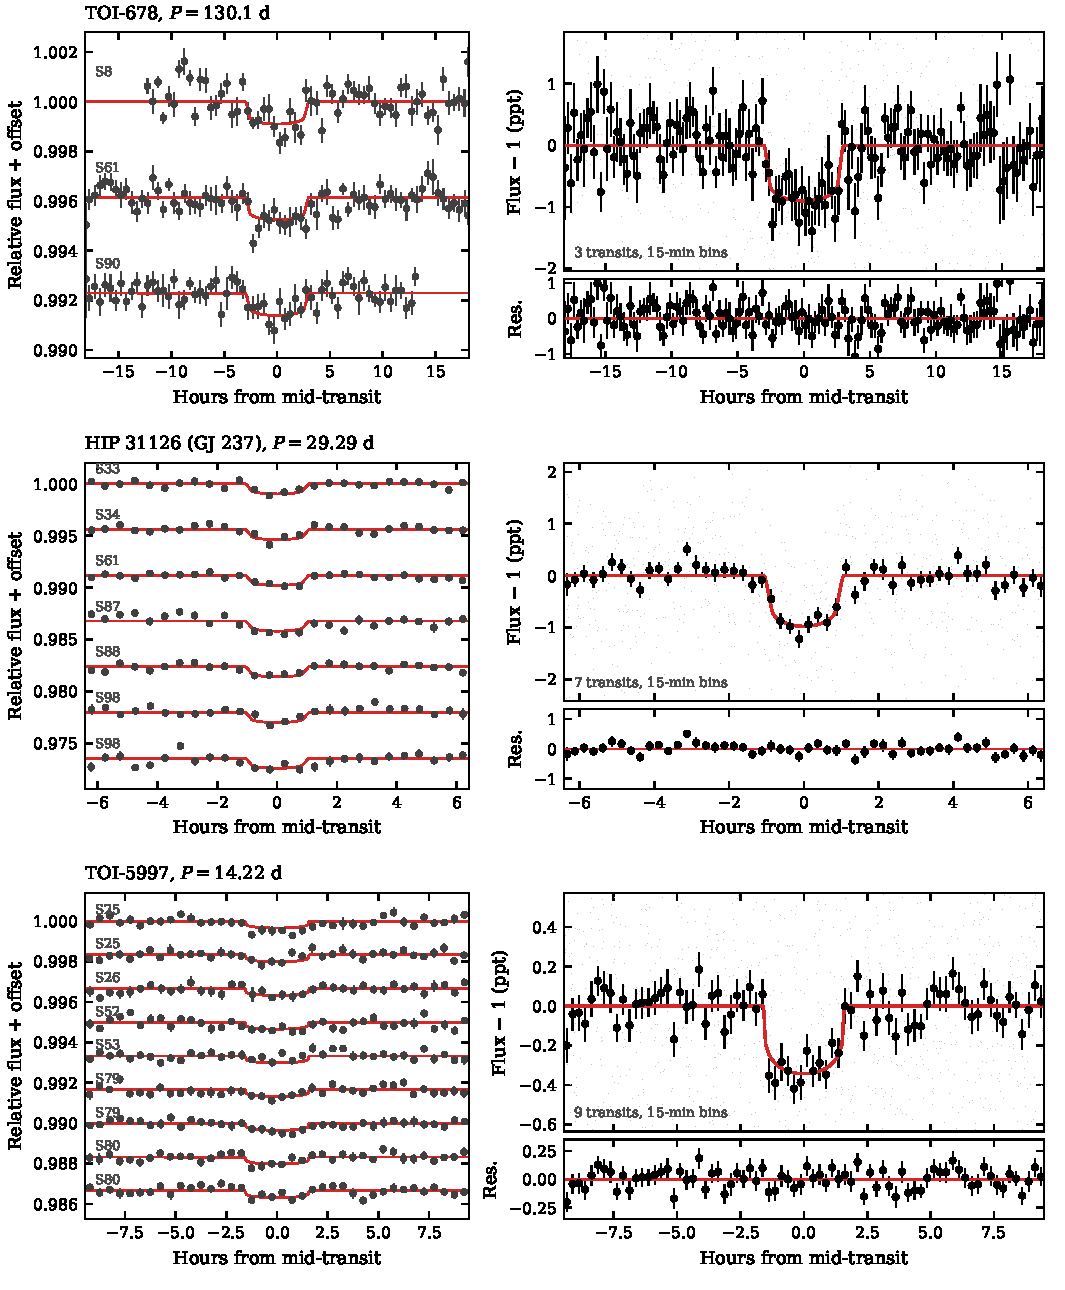
\includegraphics[width=\textwidth]{fig_transits.pdf}
\caption{TESS 2-min photometry of the three candidates. Left: each transit used,
in 30-min bins, offset vertically and labelled with its sector. Right: all of
them phase-folded, with 2-min data (grey), 15-min bins (black) and the adopted
model (red; for HIP~31126, the model for host A including the factor $g_A$),
and the residuals.}
\label{fig:lc}
\end{figure*}

\begin{table*}
\caption{Tests of the candidates. Depths are box depths in PDCSAP flux, in ppm; their uncertainties include the full-phase $\beta$.}
\label{tab:vet}
\centering
\footnotesize
\begin{tabular}{lccc}
\hline\hline
Test & TOI-678 (130.1\,d) & HIP 31126 (29.29\,d) & TOI-5997 (14.22\,d) \\
\hline
Transits used & \ntrTs & \ntrHp & \ntrTf \\
Box depth & $\boxdepTs$ & $\boxdepHp$ & $\boxdepTf$ \\
$\beta$: full phase; time averaging & \betaTs; \betacTs & \betaHp; \betacHp & \betaTf; \betacTf \\
S/N: full-phase $\beta$; time-averaging $\beta$ & \snrfullTs; \snrTs & \snrfullHp; \snrHp & \snrfullTf; \snrTf \\
Depth at random phases: significance; deeper & $\nullzTs\sigma$; 0 of \nullnTs & $\nullzHp\sigma$; 0 of \nullnHp & $\nullzTf\sigma$; 0 of \nullnTf \\
Per-transit depths, $p$ ($\chi^2$/dof): full phase; time averaging & \ptpTs\ (\ptchiTs/\ptdofTs); \ptpcTs & \ptpHp\ (\ptchiHp/\ptdofHp); \ptpcHp & \ptpTf\ (\ptchiTf/\ptdofTf); \ptpcTf \\
Per-season depths, $p$: full phase; time averaging & one transit per season & \seapHp; \seapcHp & \seapTf; \seapcTf \\
Odd; even depth & $\oddTs$; $\evenTs$ & $\oddHp$; $\evenHp$ & $\oddTf$; $\evenTf$ \\
Odd--even difference ($\sigma$) & \oeTs & \oeHp & \oeTf \\
Depth at phase 0.5$^{a}$ & $\secTs$ & $\secHp$ & $\secTf$ \\
Deepest dip elsewhere in phase ($\sigma$) & \secmaxTs & \secmaxHp & \secmaxTf \\
SAP depth; divided by CROWDSAP & $\sapTs$; $\sapcTs$ & $\sapHp$; $\sapcHp$ & $\sapTf$; $\sapcTf$ \\
Largest dip at the $P/2$ to $P/10$ epochs ($\sigma$) & $\aliasworstTs$ & $\aliasworstHp$ & $\aliasworstTf$ \\
Blind search: rank (period range searched) & not in top 5 (1--150\,d)$^{b}$ & 1 (1--60\,d) & 1 (1--40\,d) \\
Centroid shift, column; row ($\sigma$) & $\nshiftcolTs$; $\nshiftrowTs$ & $\nshiftcolHp$; $\nshiftrowHp$ & $\nshiftcolTf$; $\nshiftrowTf$ \\
Pixel-level source position ($''$, E; N) & $\offTs$ ($\pm\offsdTs$) & $\offHp$ ($\pm\offsdHp$) & $\offTf$ ($\pm\offsdTf$) \\
Target from fitted position: Mahalanobis; $\chi^2$ ($\sigma$) & \pixsigTs; \pixsigcTs & A: \pixsigHp; \pixsigcHp\ \ B: \pixsigHpBstar; \pixsigcHpBstar & \pixsigTf; \pixsigcTf \\
Neighbours able to cause the signal; excluded & \nnbTs; \nnbxTs & \nnbHp$^{c}$; \nnbxHp & \nnbTf; \nnbxTf \\
\hline
\end{tabular}
\tablefoot{$^{a}$The epochs at phase 0.5 are also the extra epochs of a
period $P/2$. $^{b}$See Sect.~\ref{sec:toi678}. $^{c}$Including B, which cannot be excluded.}
\end{table*}

\begin{table*}
\caption{Transit fits: posterior medians with 68\% intervals.}
\label{tab:fit}
\centering
\footnotesize
\begin{tabular}{lcccc}
\hline\hline
 & TOI-678 & HIP 31126 (host A) & HIP 31126 (host B) & TOI-5997 \\
\hline
$P$ (d) & $\PTs$ & $\PHp$ & $\PHpB$ & $\PTf$ \\
$T_0$ (BJD$_{\rm TDB} - 2457000$) & $\TzTs$ & $\TzHp$ & $\TzHpB$ & $\TzTf$ \\
$R_p/R_\star$ & $\rprsTs$ & $\rprsHp$ & $\rprsHpB$ & $\rprsTf$ \\
$a/R_\star$ & $\arsTs$ & $\arsHp$ & $\arsHpB$ & $\arsTf$ \\
Impact parameter $b$ & $\bTs$ & $\bHp$ & $\bHpB$ & $\bTf$ \\
$T_{14}$ (h) & $\TdurTs$ & $\TdurHp$ & $\TdurHpB$ & $\TdurTf$ \\
$(R_p/R_\star)^2$ (ppm) & $\depTs$ & $\depHp$ & $\depHpB$ & $\depTf$ \\
$R_p$ ($\rearth$) & $\RpTs$ & $\RpHp$ & $\RpHpB$ & $\RpTf$ \\
$a$ (au) & $\aTs$ & $\aHp$ & $\aHpB$ & $\aTf$ \\
Insolation ($S_\oplus$) & $\STs$ & $\SHp$ & $\SHpB$ & $\STf$ \\
$T_{\rm eq}$ (K)$^{a}$ & $\TeqTs$ & $\TeqHp$ & $\TeqHpB$ & $\TeqTf$ \\
$\rho_\star$ from the fit with $a/R_\star$ free (g\,cm$^{-3}$) & $\rhofreeTs$ & $\rhofreeHp$ & -- & $\rhofreeTf$ \\
Predicted mass ($\mearth$)$^{b}$ & \MpTs & \MpHp & \MpHpB & \MpTf \\
Predicted RV semi-amplitude (m\,s$^{-1}$) & \KTs & \KHp & \KHpB & \KTf \\
\hline
\end{tabular}
\tablefoot{Fitted jointly with the candidates: TOI-678.01, $P = \PTsb$\,d,
$R_p = \RpTsb\,\rearth$; TOI-5997\,b, $P = \PTfb$\,d, $R_p = \RpTfb\,\rearth$
\citep[1.45$\pm$0.14\,$\rearth$ in][]{collier2026}. Insolation and $T_{\rm eq}$
use $a$ from Kepler's third law. $^{a}$Zero albedo, full heat redistribution.
$^{b}$From the mass--radius relation of \citet{chen2017}.}
\end{table*}

\begin{figure*}
\centering
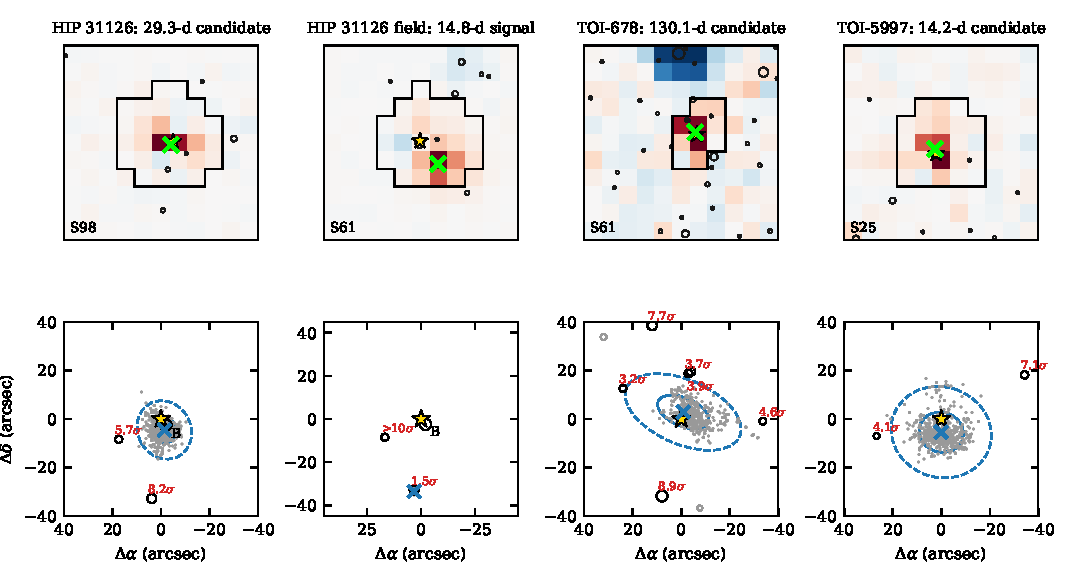
\includegraphics[width=\textwidth]{fig_pixels.pdf}
\caption{Pixel-level localisation. Top: mean difference image (out of transit
minus in transit) of the sector with the clearest signal, in the TESS pixel
frame (not north-up), with the SPOC aperture (black outline), the target
(star), other catalogued stars (circles, larger for brighter stars) and the
fitted source position (green cross). Bottom: the fitted source position on the
sky relative to the target (blue cross) with 1$\sigma$ and 3$\sigma$ contours
from the bootstrap (grey dots), and the stars able to produce the signal,
labelled with their Mahalanobis distance from the fitted position (grey circles: stars too faint to produce it). The second column spans $\pm45''$, the others $\pm40''$. The second
column is a control: the 14.8-d signal of the CTOI TIC~293689267.01, which the
fit places on a $T = 13.4$ star $33''$ south of HIP~31126.}
\label{fig:pix}
\end{figure*}

\subsection{TOI-678: a 130-day sub-Neptune candidate}
\label{sec:toi678}

TOI-678 shows three transits, in Sectors 8 (2019 February), 61 (2023 January)
and 90 (2025 March), with depths of $\ptdepaTs$, $\ptdepbTs$ and
$\ptdepcTs$\,ppm. The third is shallower, but the depths are consistent
($p = \ptpTs$, or $\ptpcTs$ with the time-averaging $\beta$). TOI-678.01 is
also shallower in that season (Sectors 87--90): $\deplateTsb$\,ppm, or
$\deplatepctTsb\%$ below its mean, which points to an instrumental effect
common to those sectors. The intervals between the transits are 11 and 6 times
$\PshortTs$\,d. Because the true period must divide both intervals, and 11 and 6
have no common factor, it can only be $\PshortTs$\,d or an integer fraction of
it. The 18 sectors of 2-min data rule out every fraction from $P/2$ to $P/10$
(Table~\ref{tab:vet}), and shorter periods would have produced many more
transits in the data. The transits have
the same depth in SAP flux and show no odd--even difference and no dip at
phase 0.5. The deepest dip elsewhere in the phase scan ($\secmaxTs\sigma$, at
phase $\secmaxphTs$) is consistent with chance, given about $\nindepTs$
independent trials.

Numbering the epochs from the Sector 61 transit, three other predicted
transits fall close to TESS data. Epoch $+7$ came 1.2\,d after the end of the
Sector 94 data, and epoch $-12$ 4.3\,d after the end of the Sector 3
full-frame images; TOI-678 was not observed in Sector 4. Epoch $-10$ (BTJD
1670.80, where BTJD = BJD$_{\rm TDB} - 2457000$) lies in Sector 13, observed
only in full-frame images, where the 30-min TESS-SPOC light curve \citep{caldwell2020} shows variations of
1--2\,ppt over a day, larger than the transit. A fit with the transit shape
fixed and a quadratic baseline gives a depth of $\ffiS$ times the expected one
in the TESS-SPOC PDCSAP flux, $\ffiSsap$ in its SAP flux and $\ffiQ$
in the QLP light curve \citep{huang2020,huang2020b}, so these data neither confirm nor
exclude the transit. In Sector 6, at an epoch where a period of $P/2$ would
place a transit, the TESS-SPOC light curve shows none (depth $\ffisix$ times
the expected).

Our blind search of all 18 sectors does not put the 130-d signal at the top:
with only three transits, several peaks of similar power appear between
$\blindloTs$ and $\blindhiTs$\,d, and the unmasked 0.8-d biweight filter used
for the blind search removes part of a 6-h transit. Without the SPOC detection
our search would not have found it. At its ephemeris the signal is deeper than
at any of the 3000 random phases ($\nullzTs\sigma$).

The pixel analysis places the source $\pixsigTs\sigma$ from TOI-678. Once
the correlated pixel noise is calibrated, however, the transit is detected in
the difference images at only $\pixdetcTs\sigma$. The calibrated $\chi^2$ test
therefore cannot exclude any star at $3\sigma$, and no neighbour is excluded by
both tests. The closest neighbours, TIC~766625715 ($T = \TTsn$, $\sepTsn''$) and
TIC~294395924 ($T = \TTsp$, $\sepTsp''$), are $\sigTsn\sigma$ and
$\sigTsp\sigma$ from the fitted position by the bootstrap test but only
$\sigcTsn\sigma$ and $\sigcTsp\sigma$ by the calibrated $\chi^2$; they would
need eclipses of $\needTsn\%$ and $\needTsp\%$ of their light. The transit duration is consistent with a
planet around TOI-678: the free fit gives $\rho_\star = \rhofreeTs\gcc$,
$\rhofreesigTs\sigma$ from the value in Table~\ref{tab:stars}. The candidate has $R_p =
\RpTs\,\rearth$ on a $\aTs$-au orbit, where it receives $\STs\,S_\oplus$ and
has an equilibrium temperature of $\TeqTs$\,K.

TOI-678.01, fitted jointly, has $R_p = \RpTsb\,\rearth$, consistent with its
TOI value of $3.4 \pm 0.3\,\rearth$. The 6.56-d TCE reaches only S/N $\snrTst$ with the time-averaging
$\beta$, below our threshold of 10, and we do not consider it here
(Appendix~\ref{app:controls}).

TRICERATOPS gives $\mathrm{FPP} = \FPPTs$ and $\mathrm{NFPP} = \NFPPTs$
(Table~\ref{tab:fpp}). Most of the NFPP ($\pnbqTs$) comes from
TIC~294395934 ($T = \TTsq$, $\sepTsq''$), which would need an eclipse of only
$\needTsq\%$; the bootstrap test puts it $\sigTsq\sigma$ from the fitted
position, the calibrated $\chi^2$ test only $\sigcTsq\sigma$. Without the
contrast curves the FPP is $\FPPtessTs$.

\subsection{HIP 31126 (GJ 237): a small planet candidate around one of two M dwarfs}
\label{sec:hip}

Seven transits of HIP~31126 in six sectors between 2021 January and 2025
December have consistent depths ($p = \ptpHp$ per transit and $\seapHp$ per
season; $\ptpcHp$ and $\seapcHp$ with the time-averaging $\beta$), no
odd--even difference and no secondary eclipse. A blind search ranks the
29.29-d period first, with a BLS S/N of $\blindsdeHp$ against $\blindnextHp$
for the next peak. The SAP depth divided by the SPOC flux fraction,
$\sapcHp$\,ppm, agrees with the PDCSAP depth. The signal is not a half-period
alias: at the extra epochs of $P/2$ the flux is slightly higher
($\secHp$\,ppm), not lower.

The difficulty is the host. A and B are $3.3''$ apart, a sixth of a TESS
pixel, and both lie inside the aperture. The fitted source position is
$\pixsigHp\sigma$ (bootstrap) and $\pixsigcHp\sigma$ (calibrated $\chi^2$)
from A, and $\pixsigHpBstar\sigma$ and $\pixsigcHpBstar\sigma$ from B, so the
pixel analysis cannot tell them apart. All \nnbxHp\ other stars able to produce
the signal are excluded; the nearest (TIC~293689268, $19''$) is at
$\nbxsigHp\sigma$ and $\nbxsigcHp\sigma$. Nor does the transit shape separate them. With A's
density the fit needs an impact parameter $b = \bHp$, and with B's density
$b = \bHpB$. The fit with free density gives $\rho_\star = \rhofreeHp\gcc$,
$\rhofreesigHpA\sigma$ from A and $\rhofreesigHpB\sigma$ from B. The candidate
would have $R_p = \RpHp\,\rearth$ and receive $\SHp\,S_\oplus$ if it orbits A,
and $R_p = \RpHpB\,\rearth$ and $\SHpB\,S_\oplus$ if it orbits B.

TRICERATOPS reflects this. A planet on A carries $\pplanetHp$ of the
probability and a planet on B $\pNTPBHp$. Eclipsing-binary scenarios together
carry $\pEBHp$, mostly on two neighbours that the pixel analysis excludes;
with those exclusions they carry $\pEBpixHp$. The FPP of $\FPPHp$ therefore mostly reflects the
unknown host: it is essentially the probability that the candidate does not
orbit A. The probability that the signal is a planet in the HIP~31126 system
is $\psysHp$.

The pixel analysis also locates the source of the 14.8-d signal in the same
light curve, a strong SPOC TCE (S/N\,32) that was submitted as a CTOI on B by
R.~Cloutier in 2019 June using the ORION pipeline \citep{cloutier2019}. Its
source is $\fsrcsig\sigma$ from TIC~\fsrcTIC, a $T = \fsrcT$ star
$\fsrcsep''$ south of A, and more than $10\sigma$ from A and B
(Fig.~\ref{fig:pix}). That star would need a $\fsrcneed\%$ eclipse. The signal
also has an odd--even difference of $\oeHpf\sigma$ in our reduction, and the
SPOC fit gives it a 5.5-h duration, longer than a planet could transit A or B
at this period (at most $\fmaxdurA$ and $\fmaxdurB$\,h). The CTOI is most
likely an eclipsing binary on that neighbour, and it does not affect the
29.29-d candidate.

\subsection{TOI-5997: a second small planet candidate}
\label{sec:toi5997}

TOI-5997 shows nine transits of the 14.216-d signal in three seasons, with
consistent depths ($p = \ptpTf$ per transit, or $\ptpcTf$ with the
time-averaging $\beta$; $p = \seapTf$ per season), no odd--even difference, no
dip at phase 0.5, and the same depth in SAP flux. A tenth transit, at BTJD
$\tenthTf$, overlaps a transit of TOI-5997\,b whose mid-time is $\tenthdtTf$\,h
later; it is masked in the light-curve tests but used in the joint fit and the
pixel analysis. A blind search
over 1--40\,d ranks the signal first; the second peak is its own half-period
alias. Both TOI-5997\,b and the candidate are shallowest in Sectors
52--53 ($\depfiveTfb$ and $\depfiveTf$\,ppm, against $\boxdepTfb$ and
$\boxdepTf$\,ppm in all sectors), again suggesting a sector-dependent
effect.

The candidate has $R_p = \RpTf\,\rearth$ and $b = \bTf$, and the free fit gives
$\rho_\star = \rhofreeTf\gcc$, $\rhofreesigTf\sigma$ from the stellar value. TOI-5997\,b, fitted
jointly, has $R_p = \RpTfb\,\rearth$, in agreement with \citet{collier2026}.
The pixel analysis places the source $\pixsigTf\sigma$ from TOI-5997. As for
TOI-678, the transit is detected in the difference images at only
$\pixdetcTf\sigma$ after calibration, so no neighbour is excluded by both tests.
The nearest, TIC~\nbTICTf\ ($T = \nbTTf$, $\nbsepTf''$), is $\nbsigTf\sigma$
from the fitted position by the bootstrap test but only $\nbsigcTf\sigma$ by
the calibrated $\chi^2$. For TOI-5997\,b, which is detected at
a similar level but needs a smaller correction for correlated pixel noise, all
four neighbours are excluded ($\pixdetcTfb\sigma$ calibrated detection).

The {`}Alopeke and PHARO images rule out companions brighter than $\Delta m
\approx 7$ beyond $0.5''$ and $\Delta m_{832} \approx 4.6$ beyond $0.1''$, so an
undetected companion beyond $0.1''$ would add at most about 1.5\% of the
light and change the
radius by less than 1\%. The star's Hipparcos--Gaia proper-motion anomaly is
not significant \citep[S/N of 2.1;][]{zhang2024}. TRICERATOPS gives
$\mathrm{FPP} = \FPPTf$ and $\mathrm{NFPP} = \NFPPTf$; for TOI-5997\,b the same
configuration gives $\FPPTfb$. Both values for the candidate are below the
thresholds commonly used for statistical validation (Sect.~\ref{sec:disc}).

\begin{table*}
\caption{False-positive probabilities from TRICERATOPS.}
\label{tab:fpp}
\centering
\footnotesize
\begin{tabular}{lccc}
\hline\hline
 & TOI-678 (130.1\,d) & HIP 31126 (29.29\,d) & TOI-5997 (14.22\,d) \\
\hline
\multicolumn{4}{l}{\emph{Adopted: archival imaging; mean and standard deviation of \nrunTs, \nrunHp\ and \nrunTf\ runs}} \\
FPP & $\FPPTs$ & $\FPPHp$ & $\FPPTf$ \\
NFPP & $\NFPPTs$ & $\NFPPHp$ & $\NFPPTf$ \\
Planet on the target (TP + PTP + DTP) & $\pplanetTs$ & $\pplanetHp$ & $\pplanetTf$ \\
Planet on an unresolved companion (STP) & $\pSTPTs$ & $\pSTPHp$ & $\pSTPTf$ \\
Planet on a resolved neighbour (NTP) & $\pNTPTs$ & $\pNTPBHp$ (on B) & $\pNTPTf$ \\
All eclipsing-binary scenarios & $\pEBTs$ & $\pEBHp$ & $\pEBTf$ \\
\hline
\multicolumn{4}{l}{\emph{Imaging and pixel-level exclusions (one run for HIP~31126)}} \\
FPP & $\FPPpixTs$ & $\FPPpixHp$ & $\FPPpixTf$ \\
NFPP & $\NFPPpixTs$ & $\NFPPpixHp$ & $\NFPPpixTf$ \\
\hline
\multicolumn{4}{l}{\emph{TESS only: no imaging, no pixel-level exclusions (one run, $2\times10^5$ draws)}} \\
FPP & $\FPPtessTs$ & $\FPPtessHp$ & $\FPPtessTf$ \\
\hline
\end{tabular}
\tablefoot{Scenario names follow \citet{giacalone2021}. No neighbour of TOI-678 or
TOI-5997 is excluded by both pixel-level tests, so for them this configuration is
the adopted one. With the adopted configuration,
TOI-678.01 has $\mathrm{FPP} = \FPPTsb$ and TOI-5997\,b $\FPPTfb$.}
\end{table*}

%%%%%%%%%%%%%%%%%%%%%%%%%%%%%%%%%%%%%%%%%%%%%%%%%%%%%%%%%%%%%%%%%%%%%%%%%%%%%%%
\section{Discussion}
\label{sec:disc}

\subsection{How strong are the candidates?}

Each signal is a SPOC detection that we recover with consistent depths in
seasons separated by up to six years, in SAP as well as PDCSAP flux, without
odd--even differences, secondary eclipses or aliases, and from a position
consistent with the target. Two lie in systems that already host a planet or
candidate, which raises their prior probability \citep{lissauer2012}. We do not
call them validated, for three reasons. Their S/N is modest: 8--10 with the
conservative noise estimate. All three pass the S/N threshold of 10 that we set
beforehand, but only with the time-averaging $\beta$. The TOI-678 candidate rests on three transits,
and our own blind search would not have found it. And the usual TRICERATOPS
validation thresholds, $\mathrm{FPP} < 0.015$ and $\mathrm{NFPP} < 10^{-3}$
\citep{giacalone2021}, are met only by the TOI-5997 candidate
(Table~\ref{tab:fpp}). We still list that one as a candidate: its S/N is the
lowest of the three, and TRICERATOPS assumes the signal is astrophysical, so
it does not test for an instrumental false alarm. One more season of TESS or
CHEOPS photometry at the predicted times would settle this. For HIP~31126 the host is unknown, which leaves the
candidate's radius uncertain by a factor of $\radratio$ and its insolation by a
factor of $\insratio$.

\subsection{Observations that would validate them}
\label{sec:followup}

Table~\ref{tab:ephem} lists the next transits.

\emph{HIP~31126.} The pair is $3.3''$ apart, so seeing-limited photometry with
point-spread-function fitting can measure A and B separately. A transit on B
would be about $\depBtrue$\,ppt deep in B's light ($V \approx 12.7$) and could
be detected or ruled out with a 1--2-m telescope in one transit. A transit on A
would be about $\depAtrue$\,ppt deep in A's light ($V \approx 10.7$) and last 2.1\,h;
detecting it needs better precision, a larger telescope or several transits. Either
way the host would be identified. Imaging closer to the star than the SOAR
limits ($\Delta I = 2.5$ at $0.15''$) would also reduce the unresolved-companion
scenarios. The expected radial-velocity semi-amplitude, about $\KHp$\,m\,s$^{-1}$
if the host is A, is within reach of ESPRESSO or NIRPS.

\emph{TOI-678.} The transit is 0.9\,ppt deep and $\TdurrTs$\,h long on a
$V = 11.6$ star near the southern ecliptic pole, out of reach of CHEOPS, and
TESS is not scheduled to observe it in its ninth year (to 2027 September).
Seeing-limited photometry of the field during a transit would test the
neighbours directly: they would need eclipses of $\needminTs$--$\needmaxTs$\%
of their own light ($\needTsq\%$ for TIC~294395934, which dominates the
NFPP), easy to detect even with partial coverage. Detecting the transit on
TOI-678 itself needs good conditions or a larger telescope. The next transits
are on \nextTsa\ and \nextTsb\ (Table~\ref{tab:ephem}).

\emph{TOI-5997.} TESS will observe TOI-5997 again in Sectors 117 and 118
(2027 May 10 to July 3; positions from \texttt{tess-point},
\citealt{burke2020}), which should cover three transits (2027 May 24, June 7
and June 21) unless they fall in data gaps. The 0.3-ppt
transit is too shallow for most ground-based telescopes but within reach of
CHEOPS. Seeing-limited photometry of the neighbours during one transit would
remove the remaining neighbour scenarios, and with a 14.2-d period there are
many opportunities each season. The radial-velocity signal, about
$\KTf$\,m\,s$^{-1}$, is small.

\subsection{The candidates in context}

Figure~\ref{fig:context} places the candidates among the
$\ntransarchive$ transiting planets in the Planetary Systems Composite
Parameters table of the NASA Exoplanet Archive \citep[DOI
10.26133/NEA13, retrieved 2026 October 8;][]{akeson2013,christiansen2025}. Only
$\ncompTs$ of them have periods longer than 100\,d, radii of 2--4\,$\rearth$ and
Sun-like hosts brighter than $V = 12$; the TOI-678 candidate ($V = 11.6$,
$T_{\rm eq} \approx \TeqrTs$\,K) would add to this small group. The HIP~31126
candidate would be a small planet in a probably bound pair of M dwarfs at 24\,pc; if it
orbits B it receives $\SrHpB$ times the Earth's insolation, and $\SrHp$ times
if it orbits A. TOI-5997 would host two small planets with a period ratio of
$\perratioTf$, $\perresoffTf$\% from the 5:2 commensurability; transit-timing
variations, if present, would be small.

\begin{figure}
\centering
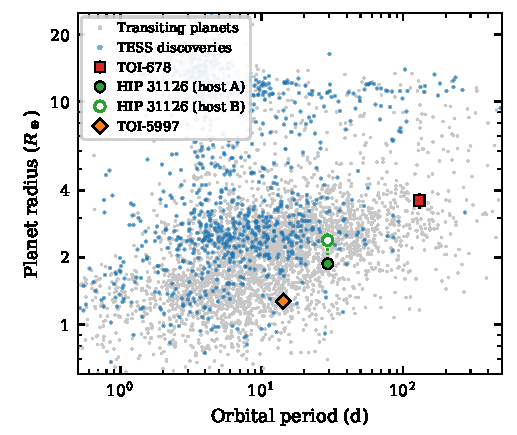
\includegraphics[width=\columnwidth]{fig_context.pdf}
\caption{Periods and radii of transiting planets in the NASA Exoplanet Archive
(grey; TESS discoveries in blue) and of the three candidates. The two possible
radii of the HIP~31126 candidate are joined by a dotted line.}
\label{fig:context}
\end{figure}

%%%%%%%%%%%%%%%%%%%%%%%%%%%%%%%%%%%%%%%%%%%%%%%%%%%%%%%%%%%%%%%%%%%%%%%%%%%%%%%
\section{Summary}
\label{sec:summary}

\begin{enumerate}
\item Three periodic signals detected by the TESS pipeline, none of them
      a TOI, have consistent depths across transits and seasons, no odd--even
      difference or secondary eclipse, no detectable alias and the same depth
      in SAP flux. Their S/N is $\snrfullTf$--$\snrfullHp$ with the
      conservative (full-phase) noise estimate and $\snrTf$--$\snrTs$ with the
      time-averaging estimate.
\item Around TOI-678, the $\PshortTs$-d signal is a $\RpTs\,\rearth$
      candidate receiving $\SrTs\,S_\oplus$, the second candidate in the
      system. It rests on three transits; a fourth, in full-frame data, is
      inconclusive. Its FPP is $\FPPTs$.
\item Around HIP~31126 (GJ\,237), the $\PshortHp$-d signal is a planet
      candidate of $\RpHp\,\rearth$ if it orbits A or $\RpHpB\,\rearth$ if it
      orbits B. Eclipsing binaries carry $\pEBHp$ of the probability; the host
      is not known.
\item Around TOI-5997, the $\PshortTf$-d signal is a $\RpTf\,\rearth$
      candidate beside the validated TOI-5997\,b. Its FPP ($\FPPTf$) and NFPP
      ($\NFPPTf$) are below the usual validation thresholds; we keep it as a
      candidate until more data confirm the modest-S/N signal.
\item A PRF fit to TESS difference images places each signal within about
      $1\sigma$ of its target and places the 14.8-d CTOI in the HIP~31126 field
      on a neighbour, most likely an eclipsing binary. For the two signals
      weakest in the difference images (TOI-678 and TOI-5997) it does not
      exclude neighbours at $3\sigma$ once correlated pixel noise is
      calibrated.
\item Seeing-limited photometry during one transit would identify the host of
      the HIP~31126 candidate and test the neighbours of TOI-678 and TOI-5997.
\end{enumerate}

\section*{Acknowledgements}
This paper includes data collected with the TESS mission, obtained from the
MAST data archive at the Space Telescope Science Institute (STScI). Funding for
the TESS mission is provided by the NASA Explorer Program. STScI is operated by
the Association of Universities for Research in Astronomy, Inc., under NASA
contract NAS5--26555. We acknowledge the use of public TESS data from pipelines
at the TESS Science Office and at the TESS Science Processing Operations
Center, including the TCE tables of the SPOC multi-sector searches and the
TESS-SPOC and QLP full-frame-image light curves
\citep{caldwell2020,huang2020,huang2020b}. This research has made use of the Exoplanet
Follow-up Observation Program (ExoFOP; DOI: 10.26134/ExoFOP5) website and of
the NASA Exoplanet Archive, which are operated by the California Institute of
Technology, under contract with the National Aeronautics and Space
Administration under the Exoplanet Exploration Program. Some of the
observations in this paper made use of the High-Resolution Imaging instruments
Zorro and {`}Alopeke. Zorro and {`}Alopeke were funded by the NASA Exoplanet
Exploration Program and built at the NASA Ames Research Center by Steve B.
Howell, Nic Scott, Elliott P. Horch, and Emmett Quigley. Zorro and {`}Alopeke
were mounted on the Gemini South and Gemini North telescopes of the
international Gemini Observatory, a program of NSF NOIRLab, which is managed by
the Association of Universities for Research in Astronomy (AURA) under a
cooperative agreement with the U.S. National Science Foundation on behalf of
the Gemini partnership. This work used speckle imaging from the SOAR telescope
and adaptive-optics imaging obtained with PHARO at the Hale Telescope, Palomar
Observatory. We thank the observers of the TESS Follow-up Observing Program
whose imaging and spectroscopy, taken from ExoFOP, made this work possible.
This work has made use of data from the European Space Agency (ESA) mission
Gaia, processed by the Gaia Data Processing and Analysis Consortium (DPAC), and
of the Two Micron All Sky Survey. It made use of \texttt{astropy}
\citep{astropy2022}, \texttt{batman}, \texttt{emcee}, \texttt{wotan},
\texttt{TRICERATOPS}, \texttt{tess-point} \citep{burke2020},
\texttt{numpy} \citep{harris2020}, \texttt{scipy} \citep{virtanen2020} and
\texttt{matplotlib} \citep{hunter2007}.

\emph{Use of generative AI.} The analysis code, the literature checks and the
draft text were prepared with the assistance of Claude (Anthropic), a large
language model, under the author's direction, and an AI-assisted review of the
draft was carried out. Most derived numbers in the text and tables are written by a script from the
analysis outputs. The author checked the
results and takes responsibility for the content.

\section*{Data availability}
All data used here are public at MAST, ExoFOP and the NASA Exoplanet Archive.
The code, the input files with checksums, posterior samples of the transit fits
and the TRICERATOPS outputs are provided as ancillary files with the arXiv
version of this paper. The full package, which also contains the light curves
and pixel response models extracted from MAST, will be archived at Zenodo.

\bibliographystyle{aasjournal}
\bibliography{refs}

%%%%%%%%%%%%%%%%%%%%%%%%%%%%%%%%%%%%%%%%%%%%%%%%%%%%%%%%%%%%%%%%%%%%%%%%%%%%%%%
\appendix


\section{Control signals}
\label{app:controls}

Table~\ref{tab:controls} applies the same tests to four other signals in the
same light curves. TOI-678.01 and TOI-5997\,b pass them except for the
consistency of their depths: those of TOI-678.01 vary between transits and
between seasons by more than the formal errors ($p = \ptpTsb$ and $\seapTsb$),
and those of TOI-5997\,b between seasons ($p = \seapTfb$). In both stars the
candidate is also shallower in the same sectors (Sects.~\ref{sec:toi678} and
\ref{sec:toi5997}), which points to an instrumental effect common to those
sectors rather than to a property of either signal. The 14.8-d signal near
HIP~31126 comes from a neighbour and is most likely an eclipsing binary
(Sect.~\ref{sec:hip}). The
6.56-d TCE of TOI-678 has consistent depths but falls below our S/N threshold;
it may deserve attention as more data accumulate.

\begin{table}[h]
\caption{Control signals, analysed with the same code as the candidates.}
\label{tab:controls}
\centering
\footnotesize
\begin{tabular}{lcccc}
\hline\hline
 & TOI-678.01 & TOI-5997\,b & 14.8-d signal near HIP 31126 & 6.56-d TCE of TOI-678 \\
\hline
Period (d) & \PTsbx & \PTfbx & \PHpfx & \PTstx \\
Transits used & \ntrTsb & \ntrTfb & \ntrHpf & \ntrTst \\
Box depth (ppm) & $\boxdepTsb$ & $\boxdepTfb$ & $\boxdepHpf$ & $\boxdepTst$ \\
S/N: full-phase $\beta$; time-averaging $\beta$ & \snrfullTsb; \snrTsb & \snrfullTfb; \snrTfb & \snrfullHpf; \snrHpf & \snrfullTst; \snrTst \\
Depth at random phases ($\sigma$) & \nullzTsb & \nullzTfb & \nullzHpf & \nullzTst \\
Per-transit $p$; per-season $p$ & \ptpTsb; \seapTsb & \ptpTfb; \seapTfb & \ptpHpf; \seapHpf & \ptpTst; \seapTst \\
Odd--even difference ($\sigma$) & \oeTsb & \oeTfb & \oeHpf & \oeTst \\
Target from fitted pixel position: Mahalanobis; $\chi^2$ ($\sigma$) & \pixsigTsb; \pixsigcTsb & \pixsigTfb; \pixsigcTfb & $>10$; $>10$ & -- \\
Neighbours able to cause the signal; excluded & \nnbTsb; \nnbxTsb & \nnbTfb; \nnbxTfb & \nnbHpf; \nnbxHpf & -- \\
FPP (adopted configuration) & $\FPPTsb$ & $\FPPTfb$ & -- & -- \\
\hline
\end{tabular}
\tablefoot{For the 14.8-d signal, A and B are among the excluded stars; its
source is TIC~\fsrcTIC. The pixel analysis of the controls uses the target pixel
files processed for the candidates (for TOI-678.01, Sectors 8, 61 and 90 only;
for the 14.8-d signal, not Sectors 87 and 98). The 6.56-d TCE was not
localised.}
\end{table}


\section{Upcoming transits}
\label{app:ephem}

Table~\ref{tab:ephem} lists the next predicted transits of the three
candidates.

\begin{table}[h]
\caption{Predicted transits after 2026 October 15 (for TOI-5997, from the
start of its 2027 observing season).}
\label{tab:ephem}
\centering
\footnotesize
\begin{tabular}{lccrr}
\hline\hline
Star & Mid-transit (UTC) & BJD$_{\rm TDB}$ & $\sigma$ (min) & $T_{14}$ (h) \\
\hline
\csname @@input\endcsname tab_ephem
\hline
\end{tabular}
\tablefoot{From the fits of Table~\ref{tab:fit}, with timing uncertainties
multiplied by the full-phase $\beta$. The UTC times are barycentric; the
light-travel time to an observer on Earth differs by up to $\pm8$\,min.
Whether a transit is observable depends on the site.}
\end{table}

\end{document}
